
\documentclass{article} 

% Deutsch
\usepackage[german]{babel} % deutsch und deutsche Rechtschreibung
\usepackage[utf8]{inputenc} % Unicode Text 
\usepackage[T1]{fontenc} % Umlaute und deutsches Trennen
\usepackage[numberedsection,nonumberlist]{glossaries} % [numberedsection] für Inhaltsverzeichnis

\usepackage[hyphens]{url}
\usepackage{textcomp} %damit geht dann \texteuro 

%Inhaltsverzeichnis Linking ermöglichen
\usepackage[hidelinks]{hyperref}
\hypersetup{
	colorlinks,
	citecolor=black,
    filecolor=black,
    linkcolor=black,
    urlcolor=black
}

%Symbole z.B für Mathematik
\usepackage{amssymb}
%Wirklich leer bei leeren Seiten (keine Seitennummern etc.)
\usepackage{emptypage} 

%% Fonts, je ein kompletter Satz an Optionen

% Times New Roman, gewohnter Font, ok tt und serifenlos
\usepackage{mathptmx}
\usepackage[scaled=.95]{helvet}
\usepackage{courier}

% ein bisschen eine bessere Verteilung der Buchstaben...
\usepackage{microtype}

% Bilder und Listings
\usepackage{graphicx} % wir wollen Bilder einfügen
\usepackage{subfig} % Teilbilder
\usepackage{wrapfig} % vielleicht doch besser vermeiden

%%Listings für um schönen Quellcode abzudrucken%%
\usepackage{listings}
\lstset{basicstyle=\footnotesize\ttfamily, breaklines=true, columns=[l]flexible, mathescape=true, showstringspaces=false, numbers=left, numberstyle=\tiny}

%%Float%%
% Das Float Package ist für Flexibilität von Fließobjekten
\usepackage{float}

%%Seitenlayout%%
\usepackage[paper=a4paper,width=14.2cm,left=36mm,height=22cm]{geometry}
\usepackage{setspace}
%Zeilenabstände%
\linespread{1.15}
%Abstände zw. Elementen in Verzeichnissen (Inhaltsvz, Abbildungsvz, Tabellenvz etc.)
\setlength{\parskip}{0.5em}
%Entfernung der Einrückung von Abschnitten, da das im deutschen nicht üblich ist.
\setlength{\parindent}{0em}

%%Seitenmarkierungen %%
%\newcommand{\phv}{\fontfamily{phv}\fontseries{m}\fontsize{9}{11}\selectfont}
%%Schickere Header und Footer
%\usepackage{fancyhdr} 
%\pagestyle{fancy}
%\renewcommand{\chaptermark}[1]{\markboth{#1}{}}
%\fancyhead[RE,LO]{\phv \nouppercase{\leftmark}}
%\fancyhead[LE,RO]{\phv \thepage}
%%keine Seitenzahl unten
%\fancyfoot[C]{\ } 

%%Mehrere Bibliographies in einem tex Dokument verwenden%%
\usepackage{bibtopic}

%%Weitere Formatierungen im Text z.B \hl{} (Highlight) \st{} (strip through)
\usepackage{soul}

%%Tiefe Inhaltsverzeichnis%%
\setcounter{tocdepth}{3}
\setcounter{secnumdepth}{3} % alle Pakete und Einstellungen

\begin{document}

\tableofcontents
\newpage

\section{Einleitung} \label{chap:einl}
Kapitel~\ref{chap:einl} behandelt kurz die wichtigsten Funktionalitäten um ein ordentliches Dokument auzusetzen.
Listing~\ref{lst:main} zeigt ein kurzes Listing mit einer C/C++ Main-Funktion

\begin{lstlisting}[caption=C/C++ Main-Funktion, captionpos=b, label=lst:main]
int main()
{
	return 0;
}
\end{lstlisting}

Abbildung~\ref{fig:defaultgrafik} zeigt zwei Smileyfaces mit einem Beispieltext. Es sollten \hl{immer Pdf Dateien} zur Einbidung genutzt werden, da nur so kein Informationsverlust stattfindet.
\begin{figure}[H]
\centering

\includegraphics[scale=0.9]{../graphics/defaultgraphic-crop} % pdflatex ohne Endung
\caption{Die wunderbare Default Grafik (kleine Version)}
\label{fig:defaultgrafik}
\end{figure}

\section{Zitate}
Marcus Schulz hat ein hervorragendes Buch für das CI/CD Tools \textit{Jenkins} geschrieben. Es nennt sich \textit{Continuous Integration mit Jenkins}~\cite{Schulz} und wird über der Rheinwerk Verlag veröffentlicht.
Eine weitere gute Ressource ist die Online-Dokumentation~\cite{Jenkins} von \textit{Jenkins}. Diese ist sehr ausführlich und bietet für jede Frage zu spezifische Antworten.

Tabelle~\ref{tab:tabelle} stellt eine Tabelle dar, die mit LibreOffice erstellt wurde.

\begin{table}[H]
\centering
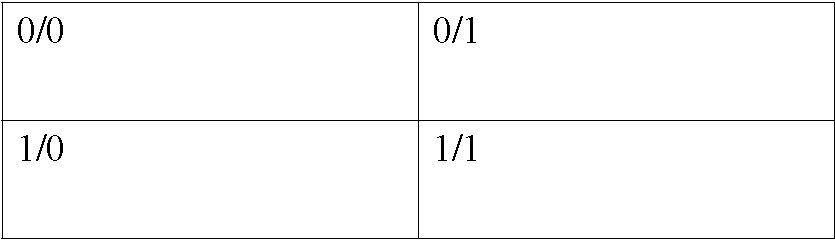
\includegraphics[scale=0.9]{../graphics/table-crop} % pdflatex ohne Endung
\caption{Eine Tabelle mit zwei Zeilen und zwei Spalten}
\label{tab:tabelle}
\end{table}

\newpage
\listoffigures % Liste der Abbildungen 
\listoftables % Liste der Tabellen
\lstlistoflistings % Liste der Listings

\bibliographystyle{plain} % Literaturverzeichnis
\begin{btSect}{physicalsources} % mit bibtopic Quellen trennen
\section*{Literaturverzeichnis}
\btPrintCited
\end{btSect}
\begin{btSect}{onlinesources}
\section*{Online-Quellen}
\btPrintCited
\end{btSect}

% dann mit "bibtex thesis1" und "bibtex thesis2" arbeiten

\end{document}
;;; Local Variables:
;;; ispell-local-dictionary: "de_DE-neu"
;;; End:
